% !TEX root = ../../Main.tex
\fancychapter{Experimental Results}
\label{Chapter:ExperimentalResults}

This chapter reports the results of the design of \Cref{Chapter:Implementation}. Seven agents were trained, one for each major currency pair. Each agent was evaluated over eleven years under the cost model of \Cref{Tables:CostModel}. Every figure below comes from a stored run that can be opened again. The analysis was computed again from those runs. It was not copied from the training logs.

The order of this chapter was chosen on purpose. The returns come first. Then come the checks that decide whether those returns mean anything, then the year that was held back, and last the result of running the seven agents together.

% !TEX root = ../../Main.tex
\section{Evaluation Protocol}
\label{Section:EvaluationProtocol}

The account, the cost model and the execution engine are described in \Cref{Section:TradingFramework} and are not repeated here. Three points are specific to the evaluation.

The evaluation window runs from 1 January 2015 to 1 January 2026, which is eleven years. It starts one year after the data begins. This way the slowest indicator in the observation, a moving average over five thousand hourly bars, is fully warmed up before the first decision.

Every result is measured from five different starting balances: $9\,900$, $10\,000$, $10\,050$, $10\,100$ and $10\,200$ euros. A strategy whose result depends on its starting point is not a real strategy. Small changes to the opening balance change the rounding of every position size, and so they change the whole sequence of trades. Reporting one balance would hide this sensitivity. The tables therefore give the mean across the five balances and the dispersion around it.

Position size is a parameter set for each pair separately. It was chosen by the sweep described in \Cref{Section:ExperimentalProcedure} and was not fixed in advance. Five pairs use the reference risk of \Cref{Equation:PositionSizing}. NZD/USD uses one and a half times that risk, and USD/JPY uses a smaller fraction of it. Position size scales every trade, but it does not change the policy that chooses the trades. The ratios, the alpha and beta decomposition and the correlation structure are therefore not affected by it.

% !TEX root = ../../Main.tex
\section{Benchmarks and Performance Metrics}

The benchmark is to buy the pair at the start of the window and hold it to the end. This is the fair comparison for a directional strategy on a single instrument. Anyone can do it, and it costs one spread. A strategy that cannot beat it does not justify its extra complexity. The thesis proposal named a random-signal baseline and a moving-average crossover instead. Both were dropped, because a trader would not hold either of them as a real alternative.

The reported metrics are those defined in \Cref{Section:PerformanceMeasurement}: total and annualised return, the Sharpe, Sortino, Calmar and Sterling ratios, maximum drawdown and the number of trades. \Cref{Tables:PerformanceMetrics} states what each one measures. All ratios use a risk-free rate of zero. They can therefore be compared across pairs without any assumption about interest rates.

% !TEX root = ../Main.tex
\begin{table}[htb!]
\centering
\footnotesize
\caption{Summary of the performance metrics used in this work.}
\label{Tables:PerformanceMetrics}
\begin{tabularx}{\textwidth}{@{}lX@{}}
\toprule
\textbf{Metric} & \textbf{Description} \\
\midrule
Net Profit & Total profit or loss \\
\addlinespace
Profit Factor & Ratio of gross profit to gross loss \\
\addlinespace
Commission and Swap & Costs that reduce net profit \\
\addlinespace
Max Balance and Equity Drawdown & Largest losses observed \\
\addlinespace
Total Trades and Winning Trades & How much the strategy trades and how often it wins \\
\addlinespace
Max Consecutive Winning and Losing Trades & How consistent the results are \\
\addlinespace
Largest Winning and Losing Trades & How large single gains or losses can be \\
\addlinespace
Average Trade & Average result per trade, a measure of trading efficiency \\
\addlinespace
Sharpe Ratio and Sortino Ratio & Risk-adjusted return \\
\bottomrule
\end{tabularx}
\end{table}

For four of them, it is worth saying why all four are reported instead of choosing one. Return says how much was made. It says nothing about the risk taken to make it. The Sharpe ratio divides return by total volatility. This penalises a strategy for moving up as much as for moving down. The Sortino ratio corrects this by counting only downside movement. Calmar and Sterling divide by drawdown instead of volatility. Calmar uses the worst loss ever suffered and Sterling the average one. They therefore measure how far the account fell, and not how volatile it was, which is the question an investor asks. A strategy can look strong on one of these and weak on another. Where that happens in this work, the text points it out.

One point applies to every number in this chapter. Returns are net of the spread quoted at the moment of each trade and of the account commission in \Cref{Tables:CostModel}. They therefore cannot be compared with results computed on bar closes with a fixed spread or with no spread. They are also lower than the same policies would show under those conditions.

% !TEX root = ../../Main.tex
\section{Results Across the Seven Majors}
\label{Section:PairResults}

\Cref{Tables:PairResults} gives the result for each pair, in alphabetical order. Total return over the eleven years goes from $+226.6\%$ on USD/CAD, the highest, to $+15.7\%$ on USD/JPY, the lowest. Every pair is profitable, and every pair is profitable from all five starting balances.

% !TEX root = ../Main.tex
\begin{table}[htb!]
\centering
\footnotesize
\caption{Result for each pair from 2015 to 2026. The return columns give the mean, standard deviation and range across the five starting balances of \Cref{Section:EvaluationProtocol}. Every pair is profitable from all five. Ratios and drawdown are from the reference run. USD/CAD returns the most, and USD/CHF is best on every risk measure.}
\label{Tables:PairResults}
\begin{tabular}{@{}lrrrrrrrrr@{}}
\toprule
\textbf{Pair} & \textbf{Mean} & \textbf{SD} & \textbf{Min} & \textbf{Max} & \textbf{Sharpe} & \textbf{Sortino} & \textbf{Calmar} & \textbf{Max DD} & \textbf{Trades} \\
\midrule
AUD/USD & 102.5\% & 10.6 & 87.2\% & 117.1\% & 0.348 & 0.496 & 0.143 & 41.1\% & 1,561 \\
EUR/USD & 73.9\% & 3.3 & 69.5\% & 77.8\% & 0.387 & 0.544 & 0.106 & 46.8\% & 1,778 \\
GBP/USD & 124.1\% & 5.1 & 115.1\% & 129.1\% & 0.397 & 0.563 & 0.155 & 50.4\% & 2,516 \\
NZD/USD & 56.4\% & 3.8 & 52.2\% & 61.7\% & 0.368 & 0.531 & 0.187 & 23.3\% & 1,011 \\
USD/CAD & \textbf{226.6\%} & 10.8 & 216.9\% & 246.0\% & 0.603 & 0.870 & 0.228 & 49.1\% & 2,213 \\
USD/CHF & 50.6\% & 5.2 & 43.4\% & 56.4\% & \textbf{0.802} & \textbf{1.552} & \textbf{0.492} & \textbf{8.2\%} & 220 \\
USD/JPY & 15.7\% & 0.7 & 14.5\% & 16.5\% & 0.251 & 0.342 & 0.057 & 24.0\% & 1,438 \\
\bottomrule
\end{tabular}
\end{table}

One fact is important for everything that follows, and it is easy to miss. \textbf{Five of the seven pairs lost value over the eleven years.} A trader who had simply bought and held would have finished down $26.1\%$ on NZD/USD, $20.3\%$ on USD/CHF, $18.2\%$ on AUD/USD, $13.5\%$ on GBP/USD and $2.9\%$ on EUR/USD. Only USD/CAD, at $+18.1\%$, and USD/JPY, at $+30.7\%$, rose. The agents made money on all seven. On five of them, the return was therefore earned in a falling market, and not in a rising one.

% !TEX root = ../Main.tex
\begin{table}[htb!]
\centering
\footnotesize
\caption{Each agent against buying and holding its own pair over the same window and under the same costs. Five of the seven pairs lost value over the eleven years, so on those the return was earned against a falling market. USD/JPY is the only pair whose benchmark rose substantially, and the only one the agent failed to beat.}
\label{Tables:Benchmark}
\begin{tabular}{@{}lrrrr@{}}
\toprule
\textbf{Pair} & \textbf{Market} & \textbf{Model} & \textbf{Excess} & \textbf{Positive Years} \\
\midrule
AUD/USD & $-18.2\%$ & $+87.2\%$ & $+105.4$ pp & 8 of 11 \\
EUR/USD & $-2.9\%$ & $+70.6\%$ & $+73.4$ pp & 5 of 11 \\
GBP/USD & $-13.5\%$ & $+129.1\%$ & $+142.5$ pp & 7 of 11 \\
NZD/USD & $-26.1\%$ & $+60.1\%$ & $+86.1$ pp & 7 of 11 \\
USD/CAD & $+18.1\%$ & $+221.0\%$ & $+202.9$ pp & 8 of 11 \\
USD/CHF & $-20.3\%$ & $+54.8\%$ & $+75.2$ pp & \textbf{10 of 11} \\
USD/JPY & $+30.7\%$ & $+16.2\%$ & $\mathbf{-14.4}$ pp & 5 of 11 \\
\bottomrule
\end{tabular}
\end{table}

The rest of this section discusses each pair in turn, in alphabetical order. For each pair it covers what the market did, what the agent returned in comparison, how that return decomposes into policy and market exposure, what the agent paid in costs, and how it traded.

\subsection{AUD/USD}

The Australian Dollar fell $18.2\%$ against the US Dollar over the eleven years. The agent returned $+87.2\%$, which is $105.4$ percentage points above holding the pair. It earned this from the short side: only $27.9\%$ of its $1\,561$ positions were long.

This result needs care in the alpha and beta decomposition. Its beta of $-2.013$ is the largest negative beta of the seven. This means that the agent was short the falling market at roughly twice its size. Of its $8.18\%$ mean yearly return, $4.96$ points are alpha and $3.22$ points are beta return, from the general fall of the market. Close to two fifths of what it earned therefore came from the Australian Dollar falling, and not from choosing when to be short. The policy does make a profit, but part of that profit would turn into a loss in a decade where the pair rose.

It trades at a moderate pace. Its median holding period is $9.7$ days, its average size is $0.77$ of the reference size, and its win rate is $52.7\%$. It made $10\,689$ euros of gross profit and paid $2\,200$ in commission. That is a $20.6\%$ share, the highest of the seven, and it comes directly from its turnover. The equity curve is uneven. Eight of eleven years are positive. The best year is 2024, at $+72.4\%$ and $81.6$ points above the benchmark, and the worst is 2017, at $-22.5\%$. Its maximum drawdown is $41.1\%$.

\begin{figure}[htb!]
\centering
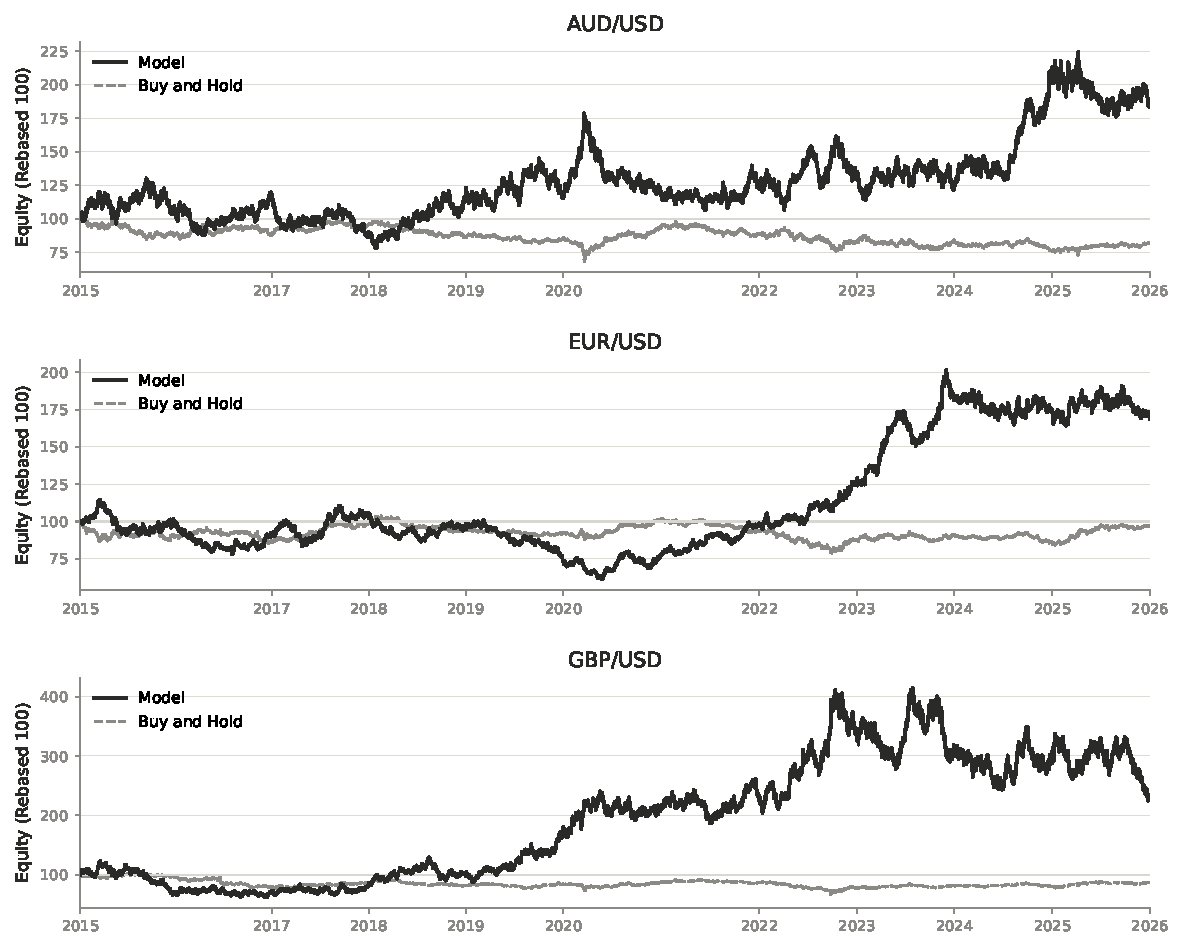
\includegraphics[width=\textwidth]{Images/PairEquityA.pdf}
\caption{AUD/USD, EUR/USD and GBP/USD against buying and holding the same pair, rebased to 100. All three benchmarks finish below their starting level.}
\label{Figure:PairEquityA}
\end{figure}

\subsection{EUR/USD}

EUR/USD is the clearest example in this work of a return that does not come from market exposure. The pair finished almost exactly where it started, down $2.9\%$ over eleven years, and the agent returned $+70.6\%$. Its beta is $+0.266$, and market exposure adds $0.01$ percentage points per year. Of a $6.63\%$ mean yearly return, $6.62$ points are therefore attributable to the policy. The market had no trend for the agent to follow, so the return came from timing alone.

It has the shortest holding period of the seven, a median of $3.9$ days, and it trades at a low $0.40$ of the reference size. Its exposure is close to balanced, with $55.5\%$ long across $1\,778$ positions. It won $51.9\%$ of them. Gross profit of $8\,734$ euros became $7\,064$ after $1\,669$ euros of commission, a $19.1\%$ share.

The equity curve in \Cref{Figure:PairEquityA} shows that the headline return also needs care here, for a different reason than on AUD/USD. Only five of eleven years are positive. The agent is roughly flat for the first six years of the window. It makes almost all of its return between 2021 and 2023, when the pair moved in unusually wide ranges: $+27.3\%$, $+29.0\%$ and $+44.0\%$ in those three years, against $-25.3\%$ in 2019. This policy needs volatility to work. Its maximum drawdown of $46.8\%$ comes from the periods when there was not enough volatility.

\subsection{GBP/USD}

GBP/USD has the highest alpha of the seven, at $+11.64\%$ per year, with a beta of $-0.054$ that is statistically indistinguishable from zero. Its mean yearly return is $11.70\%$, and only $0.06$ points of it come from market exposure. It is as close to pure policy as any result in this chapter. Sterling itself fell $13.5\%$ over the window, so the agent's $+129.1\%$ is $142.5$ percentage points above the benchmark.

It is the most active model, with $2\,516$ positions. It also holds them the longest of the six working agents, with a median of $12.6$ days. It therefore keeps many positions open at the same time, and does not trade quickly. It trades near full size, at $0.89$, and wins $51.3\%$ of the time. Gross profit was $16\,630$ euros against $3\,168$ of commission, which left $13\,462$.

Its returns come mostly from the years when sterling moved sharply. These show in \Cref{Figure:PairEquityA} as two steep sections: $+82.2\%$ in 2019 and $+52.0\%$ in 2022. \Cref{Section:TradingBehaviour} looks at the second of these in detail. The same aggressive trading also produces the worst single year of any agent, $-31.6\%$ in 2015, and the deepest drawdown, $50.4\%$. Seven of eleven years are positive. This is the most volatile of the profitable models. A reader should weigh its alpha against a drawdown that halved the account.

\subsection{NZD/USD}

The New Zealand Dollar fell the most of the seven, $26.1\%$ over the window. The agent returned $+60.1\%$, an excess return of $86.1$ points over the benchmark. Like AUD/USD, it traded mostly from the short side, with $24.0\%$ of positions long and a beta of $-0.708$.

Its alpha of $+2.79\%$ per year is the smallest of the six profitable models. Of its $4.62\%$ mean return, $1.83$ points are beta return. A large part of what it earned, though less than half, therefore came from the market falling and not from timing. By alpha and beta, it is the weakest of the six that worked.

\Cref{Figure:PairEquityB} shows it next to USD/CAD and USD/CHF. This agent is careful, and its risk numbers show the benefit. It takes the fewest positions of the active models, $1\,011$, and holds an average of $0.24$ of the reference size. Its maximum drawdown is $23.3\%$, the second lowest of the seven. Its Calmar ratio of $0.187$ is better than that of four pairs that returned much more. This shows why return is measured against drawdown, and not on its own. Gross profit was $7\,314$ euros and commission $1\,424$, a $19.5\%$ share. Seven of eleven years are positive. The best is 2022 at $+14.5\%$ and the worst is 2016 at $-6.4\%$. It is the steadiest of the models of moderate size.

\begin{figure}[htb!]
\centering
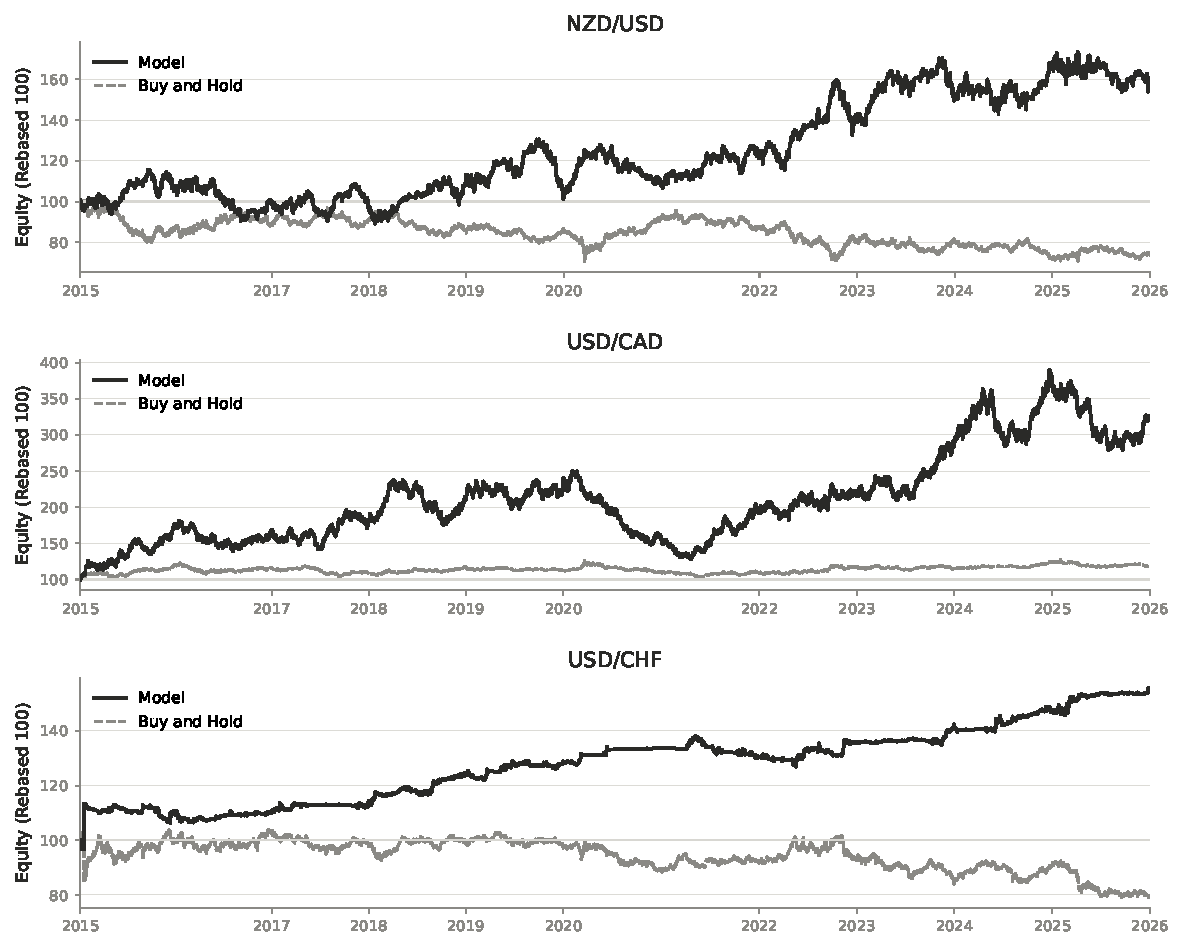
\includegraphics[width=\textwidth]{Images/PairEquityB.pdf}
\caption{NZD/USD, USD/CAD and USD/CHF against buying and holding the same pair, rebased to 100. USD/CAD is the only one of the three whose benchmark rises.}
\label{Figure:PairEquityB}
\end{figure}

\subsection{USD/CAD}

USD/CAD returned $+226.6\%$, by far the largest total in this work. It is also the result that must be read most carefully. Its beta of $+2.393$ is the highest of the seven, and the pair itself rose $18.1\%$. The agent was therefore long a rising market at more than twice its size. Of a $14.23\%$ mean yearly return, $4.21$ points are beta return and $10.02$ are alpha.

That alpha is real, and it is the second highest of the seven. So the model does not look good only because its market went up. But leverage is symmetric: it raises losses as much as gains, and the yearly record shows both. The best year is 2015, at $+71.7\%$ and $52.7$ points above the benchmark. The worst is 2020, at $-34.8\%$. Its maximum drawdown is $49.1\%$, and recovering from a $49\%$ drawdown needs a $96\%$ gain. Eight of eleven years are positive.

It is the second most active model, with $2\,213$ positions and a median holding period of $5.7$ days. It trades at $0.79$ of the reference size and has the highest win rate of the seven, at $55.0\%$. It also earned the most in euros, $25\,577$ gross, and paid $3\,432$ in commission. That is a $13.4\%$ share, lower than for the four pairs discussed above, because its profit per position was larger.

\subsection{USD/CHF}

USD/CHF returned $+54.8\%$. It is fifth of seven on return and first on every risk-adjusted measure. Its Sharpe ratio of $0.802$, Sortino ratio of $1.552$ and Calmar ratio of $0.492$ are the highest of the seven. Its maximum drawdown of $8.2\%$ is a sixth of the worst. The Swiss Franc strengthened over the period, so the pair fell $20.3\%$. With a beta of $-0.082$, the agent took almost none of that movement: of a $4.07\%$ mean yearly return, $3.91$ points are alpha.

Its trading explains all of these numbers. It takes $220$ positions in eleven years, roughly one every eighteen days. It holds an average of $0.09$ of its reference size, a tenth of what it is allowed. Because it trades so little, it pays almost nothing to trade: $130$ euros of commission against $5\,587$ of gross profit. That is a $2.3\%$ share, where the average of the seven is $16.0\%$. It keeps $97.7\%$ of what it earns, while AUD/USD keeps $79.4\%$.

It is positive in ten of eleven years, the most consistent record in this work, and its worst year is $-2.4\%$. Its win rate of $49.8\%$ is the lowest of the seven. This point deserves attention. The best model of the seven is wrong slightly more often than a coin toss. It is still the best because of how it sizes and holds the positions it gets right. It is also the only model that made money in the held-out year of \Cref{Section:OutOfSample}. On return alone it would have placed fifth and would not have been chosen. The selection criteria of \Cref{Section:ExperimentalProcedure} are there to prevent this.

\subsection{USD/JPY}

USD/JPY is the one failure of the seven, and it is the only pair whose benchmark rose by a large amount. The pair gained $30.7\%$ over the window, while the agent returned $+15.7\%$. It finished $14.4$ percentage points behind an investor who bought the pair and did nothing. Its beta of $+1.012$ and its correlation of $+0.946$ with the pair's own yearly move show what it became: a plain long position in the pair, with extra trading and extra costs. Its alpha is $-1.08\%$ per year, the only negative figure in \Cref{Tables:AlphaBeta}.

Every position it takes is long. Its median holding period is measured in years, not days. Its average action is $0.98$. This means it holds almost full size all the time and no longer makes a sizing decision at all. It earned $1\,761$ euros gross, the least of the seven, and paid $155$ in commission. Five of eleven years are positive.

\begin{figure}[htb!]
\centering
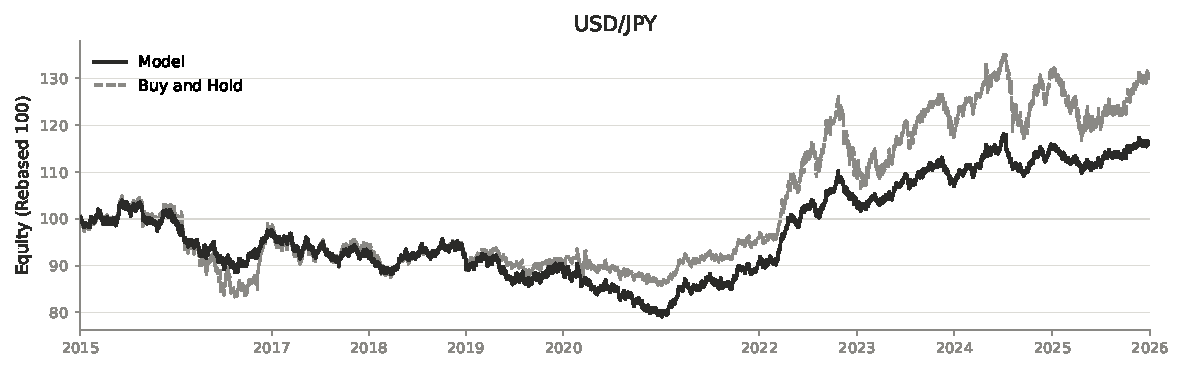
\includegraphics[width=\textwidth]{Images/PairEquityC.pdf}
\caption{USD/JPY against buying and holding the pair. The two lines move closely together. This is what a beta of $+1.012$ looks like, and it is the reason this result is reported as a failure.}
\label{Figure:PairEquityC}
\end{figure}

\Cref{Figure:PairEquityC} shows this more clearly than the statistics do: the model and the benchmark move together, with the model slightly below. \Cref{Section:NegativeResult} explains the cause and what was tried to fix it.

% !TEX root = ../../Main.tex
\section{Trading Behaviour: How the Agents Actually Trade}
\label{Section:TradingBehaviour}

A return figure says whether an agent made money. It says nothing about how, and here that matters for a specific reason. The main claim of this work is that a continuous action lets one decision set both the direction and the size of a position. If the agents had learned to use only the two ends of that action, they would be discrete traders with extra machinery, and the claim would mean nothing. This section examines what they did in practice.

\subsection{Use of the Continuous Action}

The agent outputs an action $a \in [-1, 1]$ and holds $|a|$ of the reference size defined in \Cref{Equation:PositionSizing}. \Cref{Figure:ActionDistribution} shows how this value is distributed over the whole evaluation window for each pair.

% !TEX root = ../Main.tex
\begin{table}[htb!]
\centering
\footnotesize
\caption{Trading behaviour over the evaluation window. Mean $|a|$ is the average absolute action, that is, the average fraction of the reference position size held while in the market. Win rate is the share of closed positions with a positive net result after costs.}
\label{Tables:Behaviour}
\begin{tabular}{@{}lrrrrrr@{}}
\toprule
\textbf{Pair} & \textbf{Positions} & \textbf{Long} & \textbf{Median Hold} & \textbf{Longest Hold} & \textbf{Win Rate} & \textbf{Mean $|a|$} \\
\midrule
AUD/USD & 1,561 & 27.9\% & 9.7 d & 227 d & 52.7\% & 0.77 \\
EUR/USD & 1,778 & 55.5\% & 3.9 d & 43 d & 51.9\% & 0.40 \\
GBP/USD & 2,516 & 46.9\% & 12.6 d & 149 d & 51.3\% & 0.89 \\
NZD/USD & 1,011 & 24.0\% & 5.9 d & 119 d & 52.8\% & 0.24 \\
USD/CAD & 2,213 & 65.6\% & 5.7 d & 97 d & 55.0\% & 0.79 \\
USD/CHF & 220 & 34.2\% & 8.0 d & 345 d & 49.8\% & 0.09 \\
USD/JPY & 1,438 & 100.0\% & 2,120 d & 4,004 d & 50.7\% & 0.98 \\
\bottomrule
\end{tabular}
\end{table}

\begin{figure}[htb!]
\centering
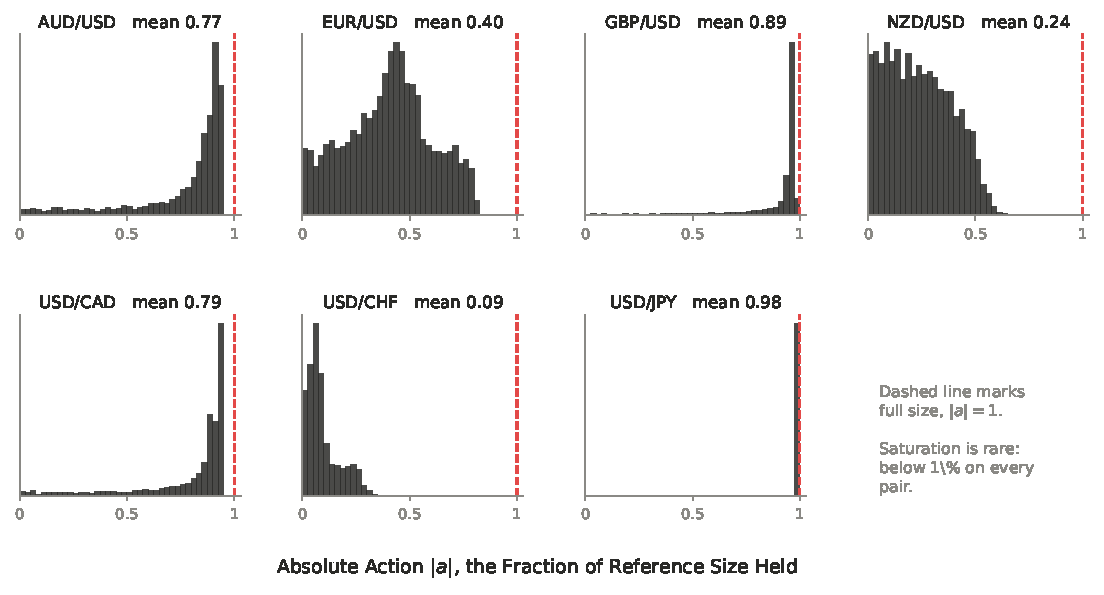
\includegraphics[width=\textwidth]{Images/ActionDistribution.pdf}
\caption{Distribution of the absolute action over the evaluation window. The dashed line marks full size. If the agents had turned the continuous action into a discrete one, these histograms would be concentrated against that line. Instead, most of the mass lies inside the range.}
\label{Figure:ActionDistribution}
\end{figure}

The action does not saturate at $+1$ or $-1$. On every pair, fewer than one percent of decisions are above $|a| = 0.98$, and on six of the seven pairs the figure is zero to one decimal place. The mean absolute action goes from $0.09$ on USD/CHF to $0.98$ on USD/JPY. The agents therefore settled on very different position sizes from the same design and the same reference risk.

This dispersion of sizes is informative in itself. USD/CHF holds roughly a tenth of the size available to it. This is why its maximum drawdown is $8.2\%$ while its Sharpe ratio is the highest of the seven. It found a small advantage and kept its size small to match, instead of pushing it harder. NZD/USD, at $0.24$, behaves in a similar way. USD/JPY is at the other end, with $0.98$. This number is the symptom of the failure described in \Cref{Section:NegativeResult}: an agent that always holds full size in one direction no longer makes a sizing decision at all.

The sizing also adapts in a second way, which the histogram does not show. The reference size is inversely proportional to the average true range, so the same action gives a smaller position when volatility rises. The action and the volatility scaling combine, and the position held is the product of the two.

\subsection{Direction, Size and Outcome Together}

\Cref{Figure:DecisionAnatomy} follows EUR/USD over three years. It shows the price, the action of the agent, the position it held as a result, and the equity that followed.

\begin{figure}[htb!]
\centering
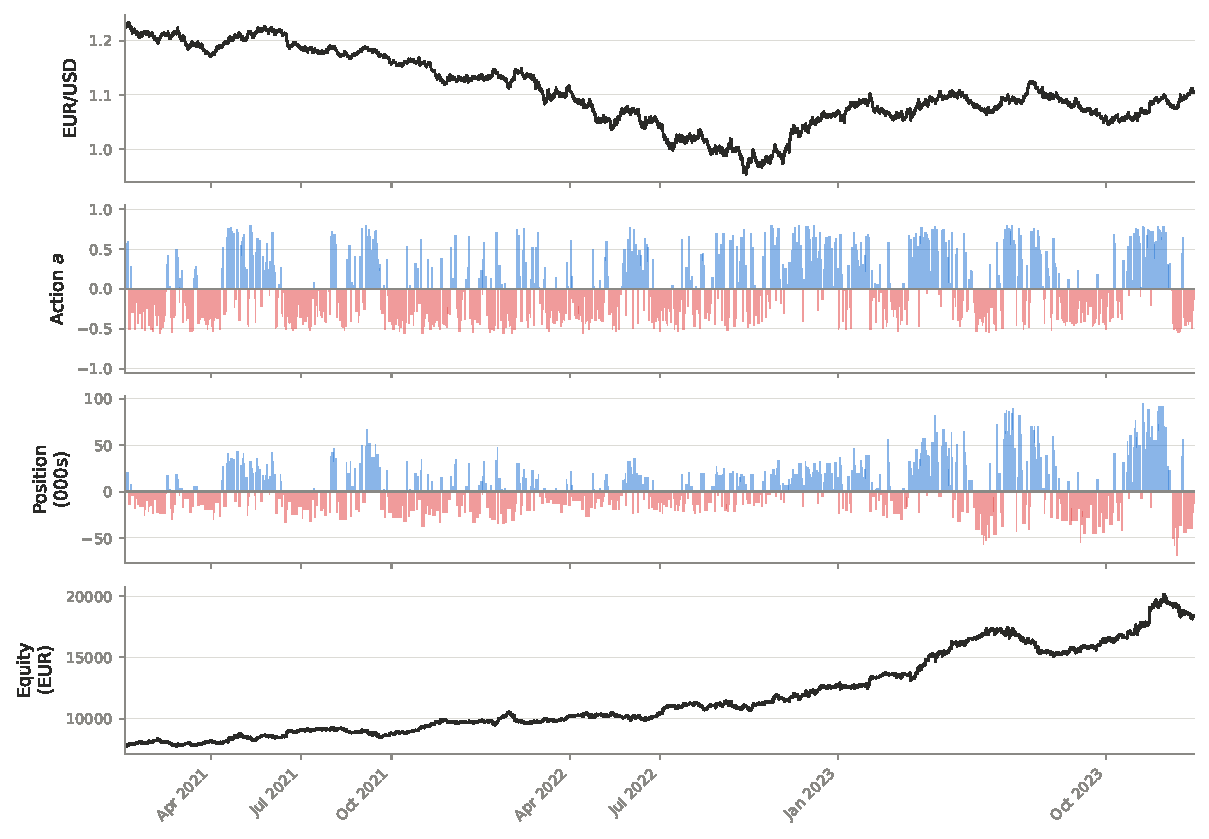
\includegraphics[width=\textwidth]{Images/DecisionAnatomy.pdf}
\caption{EUR/USD from 2021 to 2024. From top: the price; the action, positive for long and negative for short; the resulting net position in thousands of units; and account equity. The action changes sign well before the position does, because a change is only acted on when it is larger than the threshold of \Cref{Equation:Hysteresis}.}
\label{Figure:DecisionAnatomy}
\end{figure}

Three behaviours can be seen. First, the action moves continuously and does not switch between fixed levels. Its magnitude changes as much as its sign. Second, the position follows the action, but in larger steps, because the rebalance threshold blocks small adjustments. Long periods of constant position are periods where the agent kept changing its target by less than the threshold. Third, the sign does not change often. Over the three years the agent reverses direction a few dozen times. This fits the daily decision frequency, and does not fit an agent that reacts to every bar it observes.

\subsection{Trend Identification and Reversal}

The clearest example of an agent holding a position through a sustained move is GBP/USD in the second half of 2022, shown in \Cref{Figure:TrendRide}. Sterling fell from $1.22$ to below $1.04$ over roughly ten weeks, a fall of more than fifteen percent. The steepest part came after the United Kingdom fiscal announcement of late September.

\begin{figure}[htb!]
\centering
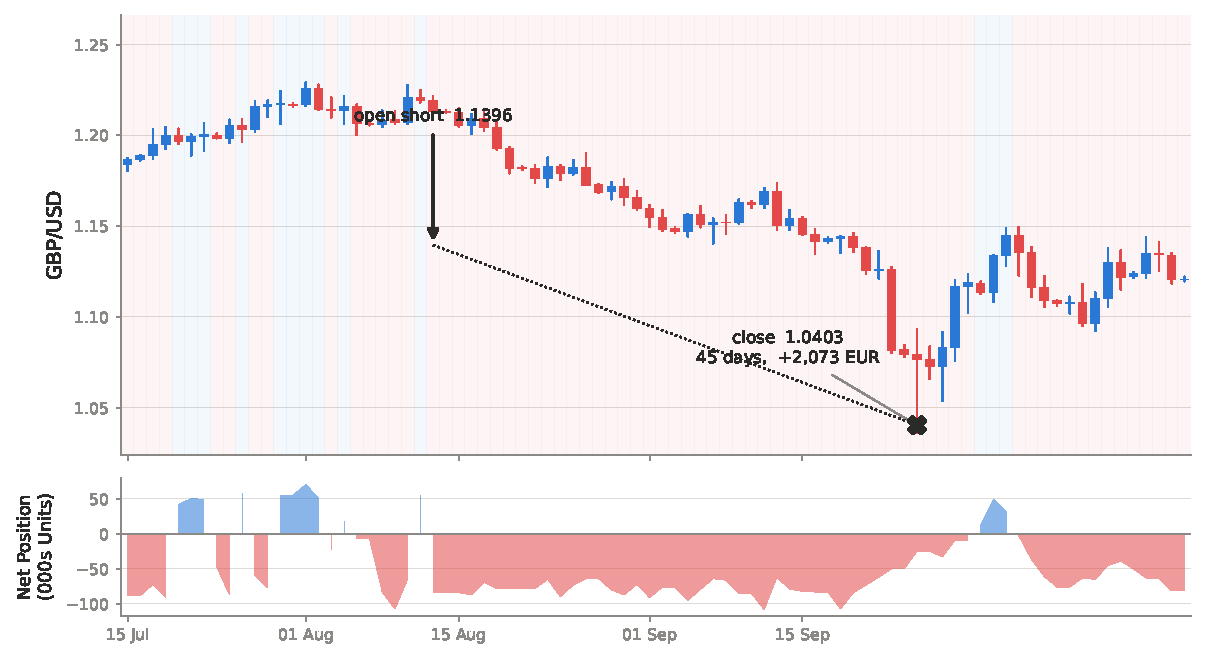
\includegraphics[width=\textwidth]{Images/TrendRide.pdf}
\caption{GBP/USD from mid-July to mid-October 2022. Background shading marks the direction of the net position, red for short and blue for long. The lower panel gives the size of that position. The marked trade is the most profitable single position of the eleven years on this pair.}
\label{Figure:TrendRide}
\end{figure}

The agent was short for almost the whole fall. It held short exposure of between fifty and one hundred thousand units, added to it as the move continued, and reduced it as the price neared the low. The marked position was opened at $1.1396$ on 12 August and closed at $1.0403$ on 26 September, forty-five days later. Its net profit was $2\,073$ euros after costs. It is the largest single position of the eleven years on this pair.

Two details are worth pointing out, because they show judgement and not luck. The agent was briefly long at the end of July, at the local high before the fall began. It was long again in the days right after the bottom. Both times the size was small. It did not hold the short position forever. Once the price recovered above $1.12$ in early October, the position was reduced and then reversed. This is how an agent behaves when it responds to the state it observes, and not when it is fixed on one direction.

\subsection{Holding Periods and Two-Sided Exposure}

\Cref{Tables:Behaviour} gives the trading statistics for each pair, and \Cref{Figure:HoldingBehaviour} shows two of them. Median holding periods go from four days on EUR/USD to nearly thirteen on GBP/USD, and the longest single positions last for months. These agents are swing traders, which hold positions for days, and not scalpers, which trade in and out quickly. This is what the daily decision frequency of \Cref{Section:ExperimentalProcedure} was meant to produce.

\begin{figure}[htb!]
\centering
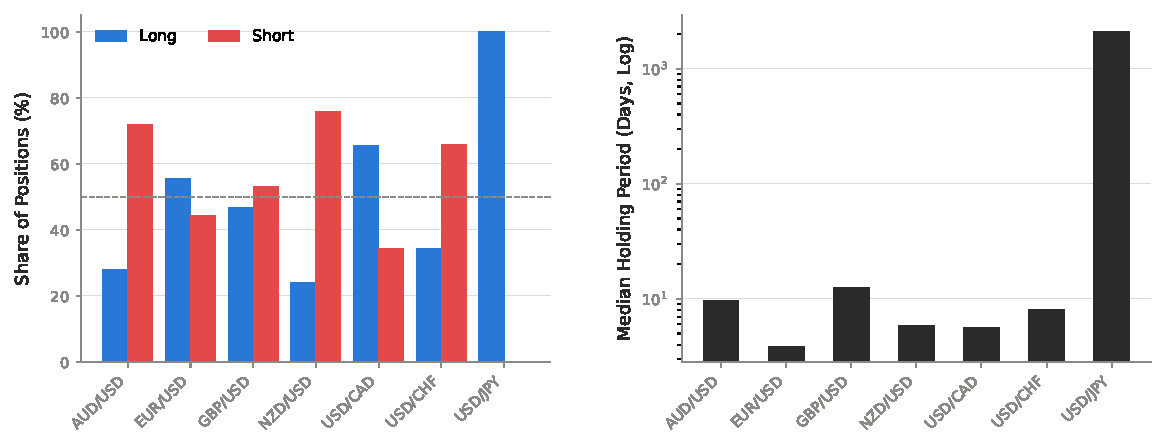
\includegraphics[width=\textwidth]{Images/HoldingBehaviour.pdf}
\caption{Left: the share of positions taken long and short. Right: the median holding period in days, on a logarithmic scale. USD/JPY is long in every position it takes and holds for years, which puts it far outside the range of the other six.}
\label{Figure:HoldingBehaviour}
\end{figure}

The long and short shares differ a lot between pairs, from $24\%$ long on NZD/USD to $66\%$ on USD/CAD. EUR/USD and GBP/USD are close to balanced. None of the six working agents trades only one side. This comes from the design and is not an accident. The eligibility test of \Cref{Section:ExperimentalProcedure} rejected any episode whose weaker side fell below a threshold, so a one-sided policy could not be selected, however profitable it looked. USD/JPY is the exception, at $100\%$ long. It is the exception because none of the $448$ seeds that were tried on that pair could pass that test.

\subsection{Where the Profit Comes From}

One statistic in \Cref{Tables:Behaviour} deserves a closer look. The win rate is the fraction of positions closed at a profit. It lies between $49.8\%$ and $55.0\%$ across the seven pairs. Six of the seven are within three points of a coin toss. USD/CHF, the best model of the seven on every risk measure, has the lowest win rate of all, at $49.8\%$.

So the agents do not make money by being right more often than they are wrong. Their profit comes from what they do with a position once it is open. They hold a larger size when the position moves in their favour than when it does not, and they keep positions that work open longer than positions that do not. A continuous action makes this possible. An agent that can only choose a direction cannot do it. This also explains how USD/CHF can be the strongest model of the seven while being wrong slightly more often than a coin toss. It trades at small size and is patient, and the few positions it holds at a larger size are the ones that worked.

\subsection{What the Trading Costs}

The engine charges the spread quoted at each fill and a real commission schedule. The difference between what the policies earned and what the account kept can therefore be measured, and does not have to be estimated.

The commission is recorded directly on every trade. The spread is not, because it is paid inside each fill and is not deducted afterwards. A buy is filled at the ask and a sell at the bid, so the cost is already included in the entry and exit prices. It can still be recovered exactly, because the two charges scale in the same way. Commission is charged at $3.5$ points per side, which is seven points for a round turn, that is, one opening and one closing trade. The spread is crossed once per round turn. Both are proportional to the traded volume, and both are converted into the account currency at the same rate. So for any position

\begin{equation}
C_{spread} = \left| C_{commission} \right| \cdot \frac{s}{7}
\label{Equation:SpreadRecovery}
\end{equation}

where $s$ is the spread in points at the moment of the trade. Applying \Cref{Equation:SpreadRecovery} to every position gives \Cref{Tables:Costs}, with $s$ taken from the recorded quotes for the month in which the position was opened.

% !TEX root = ../Main.tex
\begin{table}[htb!]
\centering
\footnotesize
\caption{What the seven agents earned before costs and what they kept, in euros. Cost share is the spread and the commission together, as a fraction of profit before costs. The mean spread column is the commission-weighted average spread paid, in points. It differs from the pair's average spread because it gives weight to the moments when the agent traded.}
\label{Tables:Costs}
\begin{tabular}{@{}lrrrrrr@{}}
\toprule
\textbf{Pair} & \textbf{Before Costs} & \textbf{Spread} & \textbf{Commission} & \textbf{Net} & \textbf{Cost Share} & \textbf{Mean Spread} \\
\midrule
AUD/USD & 11,851 & $-1,162$ & $-2,200$ & 8,488 & 28.4\% & 3.70 pts \\
EUR/USD & 9,372 & $-638$ & $-1,669$ & 7,064 & 24.6\% & 2.68 pts \\
GBP/USD & 19,086 & $-2,456$ & $-3,168$ & 13,462 & 29.5\% & 5.43 pts \\
NZD/USD & 8,552 & $-1,238$ & $-1,424$ & 5,890 & \textbf{31.1\%} & 6.09 pts \\
USD/CAD & 28,272 & $-2,695$ & $-3,432$ & 22,145 & 21.7\% & 5.50 pts \\
USD/CHF & 5,735 & $-148$ & $-130$ & 5,457 & \textbf{4.8\%} & 7.93 pts \\
USD/JPY & 2,172 & $-411$ & $-155$ & 1,606 & 26.1\% & 18.53 pts \\
\midrule
\textbf{Total} & \textbf{85,039} & $\mathbf{-8,748}$ & $\mathbf{-12,179}$ & \textbf{64,112} & \textbf{24.6\%} & --- \\
\bottomrule
\end{tabular}
\end{table}

The seven agents earned $85\,039$ euros before costs and kept $64\,112$. Of the difference, $8\,748$ euros went to the spread and $12\,179$ to commission, so \textbf{costs took $24.6\%$ of trading profit}. Commission is the larger of the two charges here because the account is a raw-spread account. On such an account the spread is narrow by design, and the broker makes its money through the commission instead. On an account with wider spreads and no commission, the same trades would have paid a similar total, split in a different way.

\Cref{Tables:Costs} has no swap column because the swap is zero on every pair. A swap-free account charges no overnight financing, so zero is the exact figure and not an approximation. This matters at these holding periods. Agents that hold positions for a median of four to thirteen days would otherwise pay financing on several hundred nights each.

The differences between pairs are large, and they follow turnover almost exactly. USD/CHF takes $220$ positions and gives up $4.8\%$ of its profit before costs, so it keeps more than nineteen euros in every twenty. NZD/USD gives up $31.1\%$ and GBP/USD $29.5\%$. A policy of the same quality therefore gives very different net results at different trading frequencies. This is why the selection criteria of \Cref{Section:ExperimentalProcedure} reward long holding periods directly, instead of relying on the return figure to include this effect. It is also why the rebalance threshold of \Cref{Equation:Hysteresis} contributes as much as \Cref{Tables:Deployment} shows.

One consequence matters for how the rest of this chapter should be read. Every return quoted in this work is net of both charges. A study that tested the same policies on bar closes with no spread and no commission would have reported the before-costs column of \Cref{Tables:Costs}. That column is a third larger, and it describes a strategy that no account could have traded.

Recovering the spread through \Cref{Equation:SpreadRecovery} works, but it is indirect and it needs a commission that is not zero. The engine computes the spread charge internally when it opens a position. It does not yet write this charge to the exported trade record as a separate field. Recording it there, next to commission and swap, is a simple improvement and is noted in \Cref{Section:FutureWork}.

% !TEX root = ../../Main.tex
\section{Path Robustness}
\label{Section:PathRobustness}

Each pair was evaluated from the five starting balances described in \Cref{Section:EvaluationProtocol}. The result is the same in every case: all seven pairs are profitable from all five entry points, thirty-five runs in total, with no exceptions. \Cref{Tables:PathRobustness} gives the individual figures.

% !TEX root = ../Main.tex
\begin{table}[htb!]
\centering
\footnotesize
\caption{Total return from each of the five starting balances, in euros. All thirty-five runs are profitable. Because broker volumes are discrete, a different opening balance rounds positions differently and produces a genuinely different sequence of trades rather than a rescaled copy of the same one.}
\label{Tables:PathRobustness}
\begin{tabular}{@{}lrrrrrrrr@{}}
\toprule
\textbf{Pair} & \textbf{9,900} & \textbf{10,000} & \textbf{10,050} & \textbf{10,100} & \textbf{10,200} & \textbf{Mean} & \textbf{SD} & \textbf{Relative SD} \\
\midrule
AUD/USD & 94.2\% & 87.2\% & 117.1\% & 108.3\% & 105.7\% & 102.5\% & 10.58 & 10.3\% \\
EUR/USD & 69.5\% & 70.6\% & 76.5\% & 77.8\% & 75.1\% & 73.9\% & 3.27 & 4.4\% \\
GBP/USD & 126.5\% & 129.1\% & 127.9\% & 122.0\% & 115.1\% & 124.1\% & 5.11 & \textbf{4.1\%} \\
NZD/USD & 61.7\% & 60.0\% & 54.4\% & 53.7\% & 52.1\% & 56.4\% & 3.76 & 6.7\% \\
USD/CAD & 230.4\% & 221.0\% & 218.5\% & 216.9\% & 246.0\% & 226.6\% & 10.81 & 4.8\% \\
USD/CHF & 56.4\% & 54.8\% & 43.4\% & 52.6\% & 45.5\% & 50.6\% & 5.16 & 10.2\% \\
USD/JPY & 15.9\% & 16.2\% & 16.4\% & 15.7\% & 14.5\% & 15.7\% & 0.69 & 4.4\% \\
\bottomrule
\end{tabular}
\end{table}

The reason this test is worth running is not obvious, so it is worth setting out. A change of one hundred euros in the opening balance looks like a change of scale, and if position sizes were continuous it would be exactly that: every trade would be one percent larger, the equity curve would be a scaled copy, and the percentage return would be identical. Sizes are not continuous. A broker accepts volume in discrete steps, so the reference volume of \Cref{Equation:PositionSizing} is rounded before an order is sent. A slightly larger balance can round a position up where a smaller one rounds it down, which changes the equity available for the next decision, which changes the size of the next position, and so on. Two runs differing only in their opening balance are therefore not the same run rescaled; after a few dozen trades they hold different positions at different times.

That the seven pairs remain profitable across all five paths, with returns clustered rather than scattered, says the results do not depend on one particular sequence of roundings. The relative standard deviation, the standard deviation divided by the mean, sits between $4.1\%$ and $10.3\%$. GBP/USD is the tightest at $4.1\%$ despite being the most active model, and AUD/USD the widest at $10.3\%$.

Two observations follow from the spread of the individual figures. The pairs with the widest relative spread, AUD/USD at $10.3\%$ and USD/CHF at $10.2\%$, are not the pairs with the largest returns; dispersion tracks how close the agent's typical position size sits to a rounding boundary rather than how much it makes. And no pair has a path that turns a profit into a loss, or even into a materially different conclusion: the worst path on USD/CAD still returns $+216.9\%$ and the best on USD/JPY still returns $+16.4\%$, so the ranking between pairs is stable across all five.

What this protocol does not measure should be stated as clearly as what it does. It varies the entry path, not the training run. Each published model is one seed drawn from a pool of between $128$ and $256$, and the variation across that pool is a different and larger source of uncertainty, addressed in \Cref{Section:StatisticalScreening} and again in \Cref{Section:OutOfSample}. A result can be perfectly stable across entry paths and still be the product of a fortunate draw.

% !TEX root = ../../Main.tex
\section{Alpha and Beta Decomposition}
\label{Section:AlphaBeta}

A currency pair moves on its own. An agent that is long a pair that happens to rise will show a profit that has nothing to do with the policy it learned. The same is true for an agent that is short a pair that happens to fall. Total return cannot separate this profit from the profit of the policy. The results are therefore decomposed into the part explained by the market and the part that is not.

For each pair, the yearly return of the model is regressed on the yearly move of the pair itself, over the eleven years from 2015 to 2025. With $r_i$ the model return in year $i$ and $m_i$ the market move in the same year, ordinary least squares gives

\begin{equation}
\beta = \frac{\sum_i (m_i - \bar{m})(r_i - \bar{r})}{\sum_i (m_i - \bar{m})^2}, \qquad \alpha = \bar{r} - \beta \bar{m}
\label{Equation:AlphaBeta}
\end{equation}

$\beta$ measures the model's exposure to the market's movement. $\alpha$ is the average yearly return that is left once that exposure is removed. The mean return then splits into an active part and a passive part:

\begin{equation}
\bar{r} = \underbrace{\alpha}_{\text{policy}} + \underbrace{\beta \bar{m}}_{\text{market exposure}}
\label{Equation:AlphaDecomposition}
\end{equation}

Yearly returns are used instead of daily returns for a specific reason. The agents hold positions for days to weeks and act once a day. A daily regression would therefore measure how the model tracks the market within a holding period. It would not measure whether the model chose the right direction over the horizon it trades. Eleven yearly observations are a small sample, and each regression coefficient has a large uncertainty. The decomposition is good enough to sort the pairs into groups, but it does not give a precise value for any one of them.

\Cref{Tables:AlphaBeta} gives both terms. Six of the seven pairs have positive alpha, and the seven fall into three clear groups.

% !TEX root = ../Main.tex
\begin{table}[htb!]
\centering
\footnotesize
\caption{Decomposition of \Cref{Equation:AlphaDecomposition}, from the yearly regression of \Cref{Equation:AlphaBeta} over 2015 to 2025. Alpha is the return attributable to the policy, and the beta return is the part explained by the pair's own movement. The two add up to the mean yearly return.}
\label{Tables:AlphaBeta}
\begin{tabular}{@{}lrrrrl@{}}
\toprule
\textbf{Pair} & \textbf{Beta} & \textbf{Alpha (\%/yr)} & \textbf{Beta Return (\%/yr)} & \textbf{Mean (\%/yr)} & \textbf{Reading} \\
\midrule
AUD/USD & $-2.013$ & $+4.96$ & $+3.22$ & $+8.18$ & Policy plus leveraged trend \\
EUR/USD & $+0.266$ & $+6.62$ & $+0.01$ & $+6.63$ & Policy, no market exposure \\
GBP/USD & $-0.054$ & $+11.64$ & $+0.06$ & $+11.70$ & Policy, no market exposure \\
NZD/USD & $-0.708$ & $+2.79$ & $+1.83$ & $+4.62$ & Policy plus leveraged trend \\
USD/CAD & $+2.393$ & $+10.02$ & $+4.21$ & $+14.23$ & Policy plus leveraged trend \\
USD/CHF & $-0.082$ & $+3.91$ & $+0.16$ & $+4.07$ & Policy, no market exposure \\
USD/JPY & $+1.012$ & $-1.08$ & $+2.64$ & $+1.57$ & No policy; the model follows the market \\
\bottomrule
\end{tabular}
\end{table}

\textbf{Three pairs have almost no market exposure.} GBP/USD, EUR/USD and USD/CHF have betas of $-0.054$, $+0.266$ and $-0.082$. Their market exposure adds $0.06$, $0.01$ and $0.16$ percentage points per year to their returns. For GBP/USD, $11.64$ of its $11.70$ points per year come from the policy. These results would hold up if the market changed direction, because they hardly depend on the direction of the market.

\textbf{Three pairs combine policy with leveraged exposure.} USD/CAD at $+2.393$, AUD/USD at $-2.013$ and NZD/USD at $-0.708$ all have a large exposure to their market, and two of them are leveraged more than two to one. Their alpha is positive in every case, so the policy adds skill on top. But between a fifth and two fifths of what they earned came from the market moving in the direction of their exposure. USD/CAD is the clearest example: $4.21$ of its $14.23$ points per year came from the pair rising while the agent was net long. If the Canadian Dollar had become stronger over the decade instead, that component would have been a loss of similar size, and the reported $+226.6\%$ would look very different.

\Cref{Figure:AlphaBeta} plots the seven together, and the three groups are clearly separate.

\textbf{One pair has no policy at all.} USD/JPY has a beta of $+1.012$ and a correlation of $+0.946$ with its own market, and its alpha is $-1.08\%$ per year, the only negative figure in the table. It is examined in \Cref{Section:NegativeResult}.

\begin{figure}[htb!]
\centering
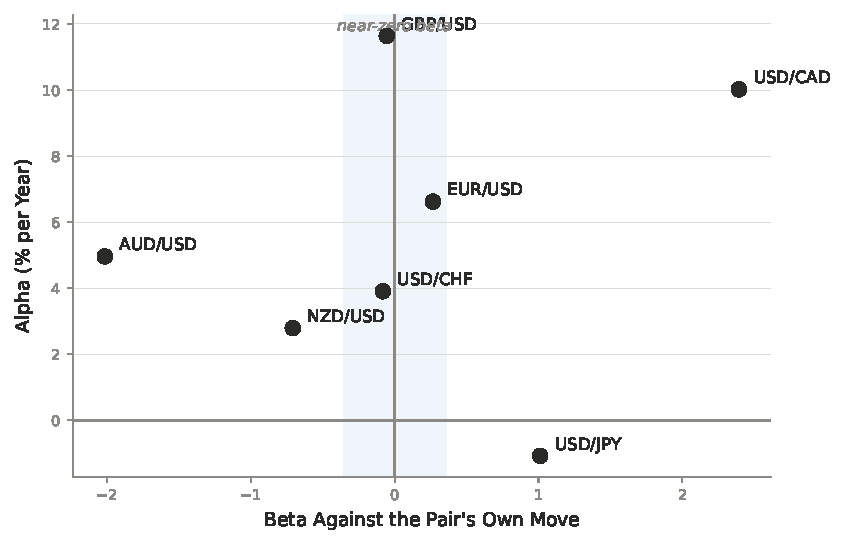
\includegraphics[width=0.82\textwidth]{Images/AlphaBeta.pdf}
\caption{Alpha against beta for the seven agents. Points inside the shaded band have almost no market exposure, so their return is attributable to the policy. USD/JPY sits at a beta of one with negative alpha. This is the pattern of a model that has copied its own market.}
\label{Figure:AlphaBeta}
\end{figure}

The method was checked before it was used. The same regression, run on the model of the previous campaign, reproduces its recorded figures exactly: a correlation of $+0.115$, a beta of $+0.130$ and an alpha of $+3.11\%$ per year. This confirms that the decomposition here is computed in the same way as the one it is compared with.

This decomposition is given priority over total return, for a reason that affects how the whole chapter should be read. The model to publish was chosen from a pool of candidates, and any measure used to make that choice is inflated by it. Return is such a measure. Beta is not. Beta describes how a policy behaves against its market. Selection can give a model a high return by luck, but it cannot give it a low beta in the same way. A large alpha with a beta near zero is therefore a stronger claim than a large return, and it is the claim this work puts first.

% !TEX root = ../../Main.tex
\section{Statistical Screening and the Rejected Candidates}
\label{Section:StatisticalScreening}

Every published model had to pass a test against a null built from the model itself. The model's own sequence of positions is rotated in time. The rotated sequence holds the same positions for the same durations, but at the wrong moments. Its regime score is therefore the score that the model's holding structure earns by luck alone. The published model must beat that score.

The null must be computed for each model and cannot be a fixed number. Across the seven pairs it goes from $48.21$ on GBP/USD to $69.82$ on NZD/USD. A fixed threshold of, say, $55$ would be below chance on one pair and well above it on another. It would accept noise in one market and reject skill in another. This was found by trying a fixed threshold first.

The screening gave a result that changes how the whole campaign should be read. \textbf{On every one of the seven pairs, the candidate with the highest return failed the test.} \Cref{Tables:BetaTraps} lists the strongest cases. A portfolio built by ranking candidates on return would have chosen models that return roughly $+250\%$ on average. Almost all of that return is market exposure, not policy.

% !TEX root = ../Main.tex
\begin{table}[htb!]
\centering
\footnotesize
\caption{Candidates rejected by the screening of \Cref{Section:StatisticalScreening}. On every pair, the candidate with the highest return failed. Ranking on return alone would have chosen these models over the ones published. They show roughly five times the return on paper, but almost none of the measurable skill.}
\label{Tables:BetaTraps}
\begin{tabularx}{\textwidth}{@{}lrrX@{}}
\toprule
\textbf{Pair} & \textbf{Return} & \textbf{$p$-value} & \textbf{Why it was rejected} \\
\midrule
AUD/USD & $+246.8\%$ & $0.146$ & Failed the screen \\
AUD/USD & $+142.6\%$ & $0.987$ & Published during the campaign, then withdrawn when the test was run \\
EUR/USD & $+141.6\%$ & --- & One-sided: long for $86\%$ of the window \\
GBP/USD & $+259.8\%$ & $0.163$ & Failed the screen \\
NZD/USD & $+253.9\%$ & $0.258$ & Failed the screen \\
USD/CHF & $+463.9\%$ & $0.973$ & Positions timed no better than the same positions shuffled; followed the franc trend \\
USD/CHF & $+341.3\%$ & $0.865$ & As above \\
\bottomrule
\end{tabularx}
\end{table}

The USD/CHF case is the clearest. A candidate that returned $+463.94\%$, more than nine times the published model, has a permutation $p$-value of $0.973$. Its positions are timed no better than the same positions shuffled. Its return came from following the trend of the franc. The published model returns a ninth of that, and it is the one with measurable skill.

Two cases are reported because they are uncomfortable. An AUD/USD candidate that returned $+142.55\%$ was published during the campaign. It was withdrawn when its $p$-value came out at $0.987$. On EUR/USD, the model in place at the time won on four of six metrics, including return, Sharpe, Sortino and drawdown. It was still replaced, because it lost on the one measure that decides whether a result is real.

This screening has limits, and they should be stated. Each published model was chosen from between $128$ and $256$ candidates, so a $p$-value near $0.05$ is close to what that many draws give by chance. Under a strict multiple-testing correction, only USD/CAD and GBP/USD, both at $0.0015$, would clearly pass. The permutation test is therefore used here as a screen that rejects bad models, which it clearly did. It is not used as a claim that the remaining models are statistically significant.

% !TEX root = ../../Main.tex
\section{Out-of-Sample Behaviour: The Held-Out Year}
\label{Section:OutOfSample}

The split of \Cref{Equation:Split} trains on 2015 to 2023, selects among episodes on 2024, and does not use 2025 at all. Because the trained weights are stored, 2025 can be scored on its own.

\textbf{The result is negative.} \Cref{Tables:TestYear} gives the figures. Five of the seven pairs lose money in 2025. The mean model return is $-6.8\%$, while the mean market move would have made money. Only USD/CHF, at $+5.0\%$, and USD/JPY, at $+0.6\%$, are positive.

% !TEX root = ../Main.tex
\begin{table}[htb!]
\centering
\footnotesize
\caption{The held-out year against the validation year and the full window. 2025 was seen by no part of the training or selection procedure; 2024 was used to choose which episode's weights were kept. The last column is the move of the pair itself in 2025.}
\label{Tables:TestYear}
\begin{tabular}{@{}lrrrr@{}}
\toprule
\textbf{Pair} & \textbf{2025 (Test)} & \textbf{2024 (Validation)} & \textbf{Full Window} & \textbf{2025 Market} \\
\midrule
AUD/USD & $-11.7\%$ & $+72.4\%$ & $+102.5\%$ & $+7.6\%$ \\
EUR/USD & $-1.2\%$ & $-5.9\%$ & $+73.9\%$ & $+13.5\%$ \\
GBP/USD & $-22.9\%$ & $-3.6\%$ & $+124.1\%$ & $+7.6\%$ \\
NZD/USD & $-5.0\%$ & $+11.0\%$ & $+56.4\%$ & $+2.8\%$ \\
USD/CAD & $-13.4\%$ & $+28.8\%$ & $+226.6\%$ & $-4.6\%$ \\
USD/CHF & $\mathbf{+5.0\%}$ & $+3.7\%$ & $+50.6\%$ & $-12.8\%$ \\
USD/JPY & $+0.6\%$ & $+7.6\%$ & $+15.7\%$ & $-0.7\%$ \\
\midrule
\textbf{Portfolio} & $\mathbf{-9.8\%}$ & --- & $+91.3\%$ & --- \\
\bottomrule
\end{tabular}
\end{table}

The comparison with 2024 is the important part, and \Cref{Figure:YearlyExcess} shows it directly. 2024 is the best year in the whole sample, with a mean excess return of $+16.4$ percentage points over the benchmark. 2025 is the worst, at $-8.7$. The difference between the two years is that 2024 was used to decide which episode's weights were kept, and 2025 was not used for anything. This gap is the measured effect of selection. It is the reason the full-window figures in \Cref{Tables:PairResults} are called an in-sample result throughout this thesis.

\begin{figure}[htb!]
\centering
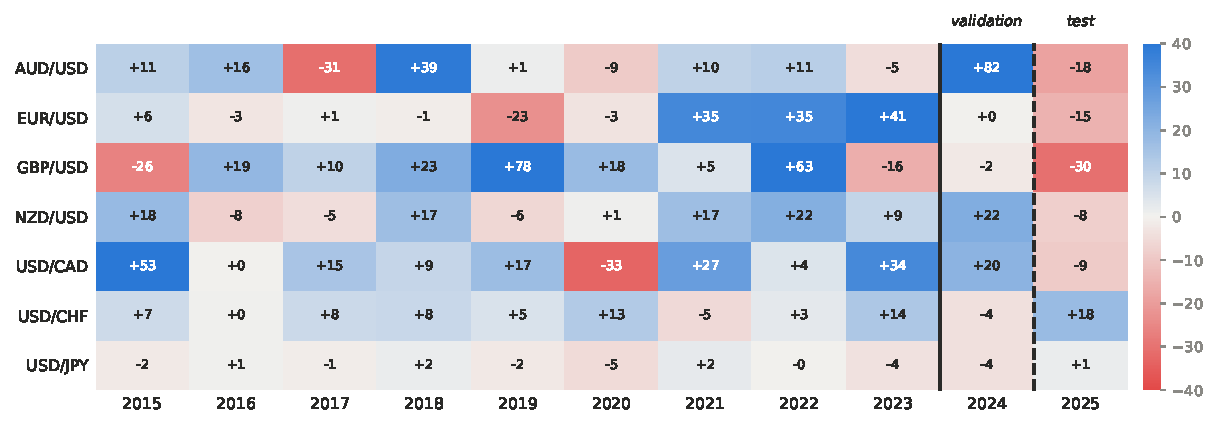
\includegraphics[width=\textwidth]{Images/YearlyExcess.pdf}
\caption{Yearly return of each agent minus the return of buying and holding the same pair, in percentage points. Blue marks outperformance of the benchmark. The solid line marks the end of the training data and the dashed line the end of the validation year, so only the last column was not seen by any part of the procedure.}
\label{Figure:YearlyExcess}
\end{figure}

There is a market explanation for the direction of the 2025 result. It is worth giving because it leads to a useful conclusion. In 2025 there was a broad dollar reversal. EUR/USD rose $13.5\%$, its largest yearly move in the eleven years, and the dollar became weaker against five of the seven pairs. The agents were trained on a decade in which the dollar mostly became stronger, and six of the seven were positioned for that. The seventh, USD/CHF, is the least directional model of the seven. It holds the fewest positions and has the lowest beta, and it is the one that made money. This agrees with the rest of the evidence and is not a coincidence. The model that depends least on the direction of the market is the one that held up when that direction changed.

The individual results should be read, and not only their average, because the models do not fail in the same way. GBP/USD is the worst, at $-22.9\%$. It is the most aggressive model of the seven. It trades near full size and has the deepest drawdown over the full window, so a year that goes against it costs a lot. USD/CAD loses $13.4\%$ and AUD/USD $11.7\%$. Both are leveraged-exposure models of \Cref{Section:AlphaBeta}, so a reversal in the direction of their beta is exactly the event that hurts them. EUR/USD loses only $1.2\%$, although the pair moved $13.5\%$. This agrees with its beta near zero: it did not take part in the reversal in either direction.

The two models that held up are the two that held the least. USD/CHF returned $+5.0\%$ while its pair fell $12.8\%$. That is an excess return of $17.8$ percentage points, and its best year against the benchmark in the whole sample. USD/JPY returned $+0.6\%$. This is not skill. It only means that the model was not exposed to the pairs that moved. Together, the two show the pattern: the models that depended least on the direction of the market were the ones that held up when that direction changed.

One year is a small sample, and no conclusion should be drawn from it beyond the obvious one. The held-out year limits what can be claimed, but it is not a final judgement on the design. The design kept trading in a sensible way on data it had never seen. It lost money doing so, in a year whose direction was not in its training data.

% !TEX root = ../../Main.tex
\section{A Negative Result: USD/JPY}
\label{Section:NegativeResult}

USD/JPY did not work, and the reason is known.

The numbers show that the model behaves like the market. Its correlation with the pair's yearly move is $+0.946$ and its beta is $+1.012$, so its exposure to the pair is almost exactly one for one. Its alpha is $-1.07\%$ per year. It returns $+15.7\%$ over the eleven years, against roughly $+25\%$ for simply buying and holding the pair. It therefore underperforms a benchmark that costs nothing to run. The model is long at every point in the window.

The cause is in the data. USD/JPY rose from roughly $120$ to $150$ over the period, and the move was concentrated and mostly in one direction. On such a series, holding a long position is close to optimal, and any change from it is punished. The reward signal therefore gives no gradient towards changing the exposure, and the agent settles on the simplest policy that follows the trend. Over the same period the other six majors mean-revert often enough that trading both sides is rewarded, and their agents learned to do it.

This was not assumed. It was tested. Across seven configurations and $448$ seeds, every run converged to a directional policy at full size. One augmentation shows the agent mirrored price series, and it was meant to remove exactly this bias. Raising it made the resulting policies more binary, not less.

The result is reported because it is informative. It shows the limit of the method. This design learns to time its exposure in markets that turn. On a market that does not turn, it ends up just holding the trend, and it pays trading costs to do so. A reader who is deciding whether to use the approach elsewhere needs to know this limit more than they need a seventh success.

% !TEX root = ../../Main.tex
\section{Portfolio: The Seven Models Combined}
\label{Section:Portfolio}

A trader would not run just one of these agents. They would run all seven. This is a different question from how each agent does alone. For a portfolio, what matters is not only what each component returns, but also whether the components lose money at the same time.

The seven published models are combined by giving each one a seventh of the capital at the start of the window, with no rebalancing afterwards. With $E_p(t)$ the equity of pair $p$ at time $t$, the portfolio is

\begin{equation}
V(t) = \frac{1}{7} \sum_{p} \frac{E_p(t)}{E_p(0)}
\label{Equation:Portfolio}
\end{equation}

By construction, the total return of such a portfolio is the mean of its components. The interesting part is therefore the risk, and not the return. \Cref{Tables:Portfolio} compares the portfolio with the average of the seven pairs taken separately.

% !TEX root = ../Main.tex
\begin{table}[htb!]
\centering
\footnotesize
\caption{The equal-weight portfolio of \Cref{Equation:Portfolio} against the average of its seven components. Return is the same by construction, so the whole effect is on risk.}
\label{Tables:Portfolio}
\begin{tabular}{@{}lrrl@{}}
\toprule
\textbf{Measure} & \textbf{Portfolio} & \textbf{Mean of the seven} & \textbf{Effect} \\
\midrule
Total return & $+91.3\%$ & $+91.3\%$ & Equal by construction \\
Annualised return & $+6.07\%$ & $+6.07\%$ & Equal by construction \\
\addlinespace
Maximum drawdown & $\mathbf{15.9\%}$ & $34.5\%$ & More than halved \\
Sharpe ratio & $\mathbf{0.632}$ & $0.451$ & Above all but USD/CHF \\
Sortino ratio & $0.906$ & $0.685$ & Improved \\
Calmar ratio & $0.381$ & $0.194$ & Nearly doubled \\
Sterling ratio & $1.059$ & $0.670$ & Improved \\
\addlinespace
Mean correlation & \multicolumn{2}{c}{$+0.062$ across all 21 pairings} & Close to independent \\
\bottomrule
\end{tabular}
\end{table}

\Cref{Figure:PortfolioEquity} plots the portfolio against its components. The maximum drawdown falls from an average of $34.5\%$ to $15.9\%$. The Sharpe ratio rises from an average of $0.451$ to $0.632$, which is above every single pair except USD/CHF. The portfolio gives the same return with less than half the worst loss.

\begin{figure}[htb!]
\centering
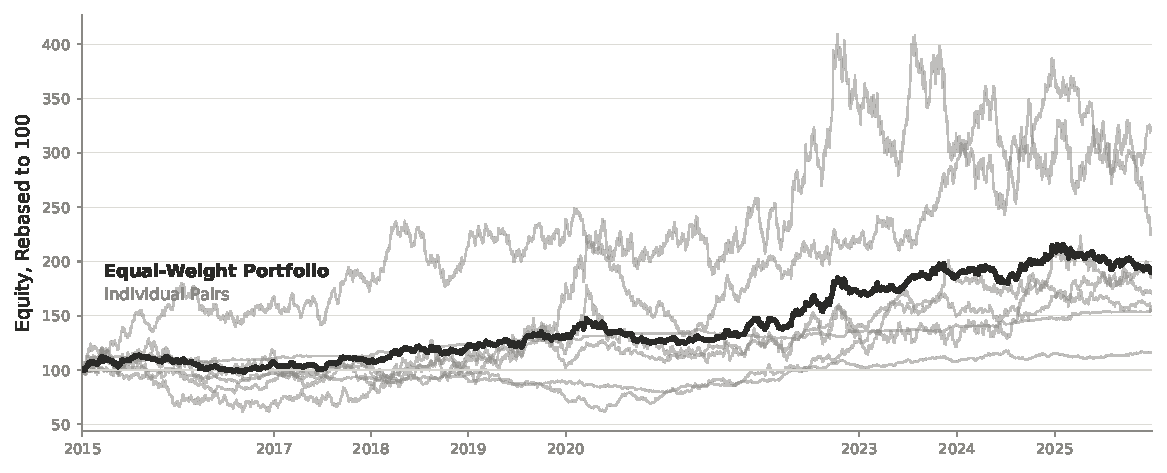
\includegraphics[width=\textwidth]{Images/PortfolioEquity.pdf}
\caption{The equal-weight portfolio against its seven components, all rebased to 100. The portfolio is smoother than any component because the components do not fall together.}
\label{Figure:PortfolioEquity}
\end{figure}

\Cref{Figure:Correlation} shows the reason. The mean correlation between the daily returns of any two of the seven models is $+0.062$, and no pair of models is above $+0.46$. Three pairings are negative. The seven agents were trained by the same procedure on seven instruments that are themselves correlated, since all of them have the US Dollar on one side. Even so, their profits and losses come at different times. This follows from the design. Each agent learned the timing of its own market, so the agents share a method but not a position.

\begin{figure}[htb!]
\centering
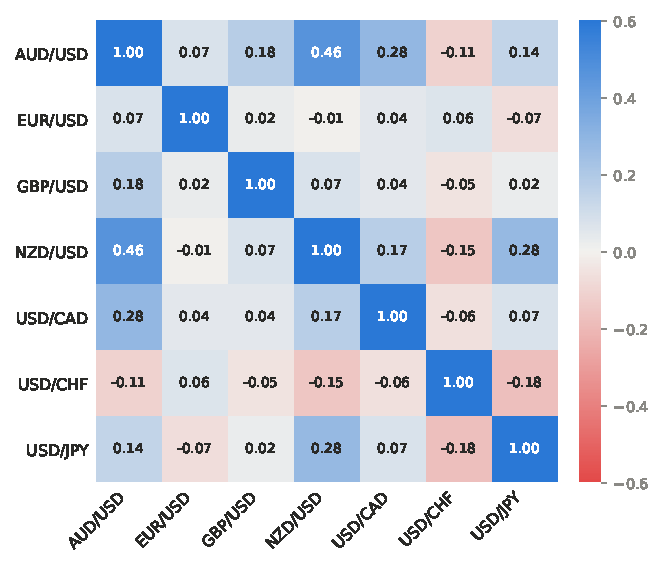
\includegraphics[width=0.68\textwidth]{Images/Correlation.pdf}
\caption{Correlation between the daily returns of the seven agents over the evaluation window. The mean of the off-diagonal entries is $+0.062$.}
\label{Figure:Correlation}
\end{figure}

\subsection{Does the Result Depend on the Position Sizes?}

As \Cref{Section:EvaluationProtocol} states, the seven models do not all run at the same position size. The portfolio above is therefore the combination as published, and it is not built on a common risk level. It is fair to ask whether this choice produces the result. The question can be checked directly.

Position size is proportional to the account balance. Multiplying the risk fraction by a constant therefore multiplies every position, and so every per-step return, by the same constant. A common-risk version can be built by rescaling each component's returns to the level it would have run at, and compounding them again. This ignores the rounding of volumes to the broker's step and any margin limit. It is an approximation and not a new run, but it is close enough to answer the question. \Cref{Tables:CommonRisk} gives both versions.

% !TEX root = ../Main.tex
\begin{table}[htb!]
\centering
\footnotesize
\caption{The equal-weight portfolio as published, against a version in which every component runs at a common risk level. The common-risk version is built by rescaling each component's per-step returns. This is exact for a strategy whose position size is proportional to balance, but it ignores volume rounding. The two differ little, so the diversification result does not depend on how positions are sized.}
\label{Tables:CommonRisk}
\begin{tabular}{@{}lrrr@{}}
\toprule
\textbf{Measure} & \textbf{As Published} & \textbf{Common Risk} & \textbf{Difference} \\
\midrule
Total return & $+91.3\%$ & $+91.6\%$ & $+0.3$ pp \\
Annualised return & $+6.07\%$ & $+6.09\%$ & $+0.02$ pp \\
Sharpe ratio & $0.632$ & $0.608$ & $-0.024$ \\
Sortino ratio & $0.906$ & $0.866$ & $-0.040$ \\
Calmar ratio & $0.381$ & $0.320$ & $-0.061$ \\
Maximum drawdown & $15.9\%$ & $19.0\%$ & $+3.1$ pp \\
\bottomrule
\end{tabular}
\end{table}

The two portfolios are almost the same. Total return moves from $+91.3\%$ to $+91.6\%$, the Sharpe ratio from $0.632$ to $0.608$, and the maximum drawdown from $15.9\%$ to $19.0\%$. The common-risk version is slightly worse on risk, as expected. Putting USD/JPY at the same risk level as the others makes its positions five times larger and takes its own maximum drawdown to roughly $80\%$. At a seventh of the capital, the portfolio absorbs even that. The conclusion of this section therefore does not depend on how the positions are sized. It depends on the correlation structure of the models, which sizing does not change.

Two limits apply to this result. As \Cref{Section:EvaluationProtocol} states, the components do not all run at the same position size. The portfolio is therefore the combination as published, and not a risk-parity allocation. Making the sizes equal would change the weights, but not the correlation structure that produces the benefit. Also, the portfolio shares the weakness of its components. In the held-out year of \Cref{Section:OutOfSample} it returns $-9.8\%$, better than five of the seven pairs and worse than two. This is what an average should do when most of its components fall together for a shared reason.

Two results matter most. First, six of the seven agents produced positive alpha against their own market. Three of those did so with a market sensitivity close to zero, and this is what separates a trading strategy from leveraged market exposure. Second, the seven agents combined behave better than any of them alone, because their returns are close to uncorrelated.

On the other hand, the held-out year is negative, and the selection is not corrected for multiple testing. \Cref{Chapter:Conclusion} sets out what these two facts allow this work to claim and what they do not.